\documentclass[20pt,a4paper]{article}
\usepackage{hyperref}
\usepackage{sectsty}
\usepackage{graphicx}
\usepackage{enumitem}
\usepackage{algorithm}
\usepackage{algorithmic}
\usepackage{amsmath}
\DeclareMathOperator*{\argmax}{argmax} % thin space, limits underneath in displays

\sectionfont{\fontsize{10}{15}\selectfont}
\subsectionfont{\fontsize{9}{15}\selectfont}
\subsubsectionfont{\fontsize{8}{15}\selectfont}


\begin{document}
% Document title
\title{Transactions Anomaly Detection with Unsupervised Learning }

\author{
          Otmazgin, Shon\\
          \texttt{305394975}\\
          \texttt{shon711@gmail.com}
          \and
          Rubin, Sapir\\
          \texttt{301659751}\\
          \texttt{rubinsapir@gmail.com}
          }
\date{March 26, 2020}
 %
\maketitle
% 

\begin{abstract}
    Supervised learning has been widely used to detect anomaly in credit
    card transaction records based on the assumption that the pattern of a
    fraud would depend on the past transaction. However, unsupervised
    learning does not ignore the fact that the fraudsters could change their
    approaches based on customers' behaviors and patterns. in this study we
    will present iterative method of using mixture of Gaussian's to detect
    anomaly in credit card transactions. We will compare it with iterative
    method using OneClassSVM. In each method our algorithm utilizes the
    model functions(likelihood and shifted from support vector) scores,
    evaluates samples with their scores and samples score under threshold T
    consider to be anomalies. the described method is iterative until model
    converges or max iteration exceeds. The data set used in this study is
    based on real-life data of credit card transaction. Due to the
    availability of the response(labels), after training the models we can
    evaluate the performance of each model. The performance of these two
    methods is discussed extensively in this paper.
\end{abstract}

\section{Data set}
    The data set that is used for credit card fraud detection is derived from
    the following
    \href{https://eur02.safelinks.protection.outlook.com/?url=https\%3A\%2F\%2Fdata.world\%2Fraghu543\%2Fcredit-card-fraud-data\&data=02\%7C01\%7CYael.Madar\%40biu.ac.il\%7Cb48189911f224aef8c2e08d79ff0c5e6\%7C61234e145b874b67ac198feaa8ba8f12\%7C0\%7C0\%7C637153728776732928\&sdata=tzNpfPA2qlY12Dp1Zli5FW5ugw0Q05OaTCay5mAvo4c\%3D\&reserved=0}{URL}
    
    The data set contains transactions made by credit cards in September
    2013 by European cardholders. This data set presents transactions that
    occurred in two days, where we have 492 frauds out of 284,807
    transactions. The data set is highly imbalanced, the positive class
    (frauds) account for 0.172\% of all transactions.
    Due to confidentiality issues, there are not provided the original
    features and more background information about the data. It contains
    only numerical input variables which are the result of a PCA
    transformation.
    
    \begin{enumerate}[label=\roman*)]
    \item
      Features V1, V2, \ldots{} V28 are the principal components obtained
      with PCA;
    \item
      The only features which have not been transformed with PCA are Time
      and Amount.
    \item
      Feature Time contains the seconds elapsed between each transaction and
      the first transaction in the data set.
    \item
      The feature Amount is the transaction amount of money spent in each transaction.
    \item
      Feature Class is the response variable and it takes value 1 in case of
      fraud and 0 otherwise.
    \item
      There is no missing data in the entire data set
    \end{enumerate}

\section{Problem statement}
The Credit Card Fraud Detection Problem includes past credit card
transactions. The need is to identify whether a new transaction is
fraudulent or not. The data is highly imbalanced and our aim here is to
detect the fraudulent transactions while minimizing the incorrect fraud
classifications. Let's realize that we are looking for a needle in a hay
barn. 99\% of the data are valid transactions. We could balance the data
by oversampling or under sampling and even to fit the models with only
valid transactions, but we want our models to be able to produce results
in the real world and not just in testing environment, therefore we will
develop our model as like labels was not existed. This is why we should
use the imbalanced data, in order to better simulate real world cases.
If our model can identify even a fraction of fraud cases with high
precision, it is adding value.



\section{Data Exploration}
    \subsection{Class Distribution}
        \begin{center}
        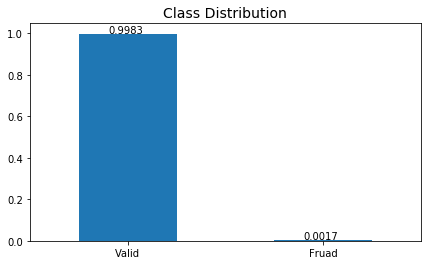
\includegraphics[scale=0.45]{graphs/output_16_0.png}
        \end{center}
        Only 492 (or 0.172\%) of transaction are fraudulent. That means the data
        is highly imbalanced with respect to the target variable Class.

    \subsection{Transactions Time and Amount Distributions}
        \begin{center}
        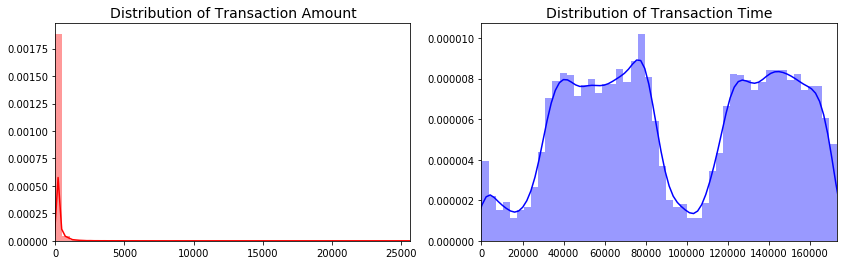
\includegraphics[scale=0.45]{graphs/output_19_0.png}
        \end{center}
        \begin{enumerate}[label=\roman*)]
          \item Most transactions are small amounts transactions, less than \$100.
          \item Clearly, it looks like there are cycles in Time.
        \end{enumerate}

        \subsubsection{Transactions Time and Amount Distributions by Class}
            \begin{center}
            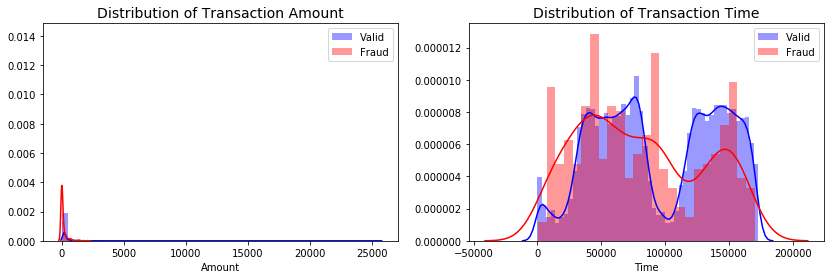
\includegraphics[scale=0.45]{graphs/output_22_0.png}
            \end{center}
            
            \begin{enumerate}[label=\roman*)]
            \item
              The `Time' feature looks pretty similar across both types of
              transactions. You could argue that fraudulent transactions are more
              uniformly distributed compared to the valid transactions which have more cyclical
              distribution. This could make it easier to detect a fraudulent
              transaction during at an `off-peak' time.
            \item
              Most transactions are small amounts, less than \$100. Fraudulent
              transactions have \$122 mean amount, standard deviation \$256 and \$2125 maximum. valid transaction have \$88 mean amount, standard deviation at \$250 and \$25691 maximum.
            \end{enumerate}
        Now let's see if the transaction amount differs between the two types.

    \begin{center}
    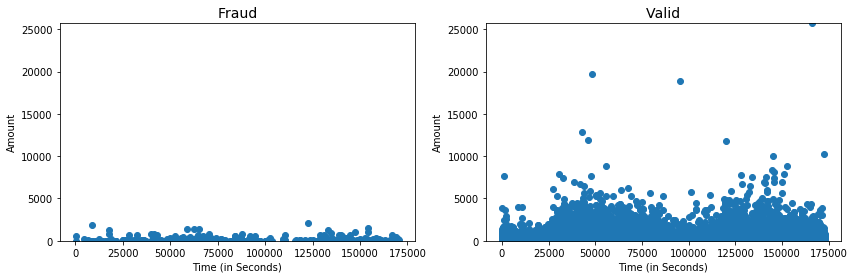
\includegraphics[scale=0.45]{graphs/output_24_0.png}
    \end{center}
    Both types equally distributed over time. y-axis is significantly different
    between fraud and valid transactions.

\textbf{Reminder} - Unsupervised Learning is a process of training a
machine learning model on a data set in which target variable is unknown.
we will develop our model as like labels was not existed.

\section{Data preprocess} 
\subsection{Scaling}
We will scale the columns comprise of Time
and Amount . Time and Amount should be scaled as the other columns
already scaled through the PCA transformation. We will use Robust
Scaler, Scale features using statistics that are robust to outliers.

\subsection{Split the Data to Train and Test}
We will take randomly fraction of the data set(20\%), this is just to save time during training, then split it to train(80\%) and test(20\%). 
Train size: (45569, 30), Test size: (11392, 30)
\section{Terms}

\begin{enumerate}[label=\roman*)]
\item
  True Positives: Correctly Classified Fraud Transactions
\item
  False Positives: Incorrectly Classified Fraud Transactions
\item
  True Negative: Correctly Classified Non-Fraud Transactions
\item
  False Negative: Incorrectly Classified Non-Fraud Transactions
\end{enumerate}

\subsection{Introduce Precision, Recall and F1 scores:}

\begin{enumerate}[label=\roman*)]
\item
  Precision: \(p=\frac{TP}{TP + FP}\)
\item
  Recall: \(r=\frac{TP}{TP + FN}\)
\item
 $F$ score: $F_1=\frac{2pr}{p+r}$
\end{enumerate}

Precision, as the name says, says how precise (how sure) is our model when it classifies a transaction as fraud transaction, while Recall is the ratio of classified fraud cases from all the fraud cases.

Precision/Recall Trade off: The more precise (selective) our model is,
the less cases it will detect.

The F1 score is the harmonic mean of the precision and recall, where an F1 score reaches its best value at 1 (perfect precision and recall) and worst at 0.

\subsection{Thresholds}
Assume $\mathbf{X}$ is the data set, $\ell(s|\theta)$ is the model score function and $\theta$ is the model estimators for unknown parameters, then $TS$ is all possible thresholds:
$$TS = [\ \ell(s|\theta)\ |\ s\ \in\ \mathbf{X}]$$ 
Select threshold for score function:
$$T = TS[ \argmax_{f \in F} f ] $$
$F$ is all possible $F_1$ scores.\\
In other words the threshold selected is where \(F_1\) score reach
the maximum.

\section{Iterative approach}

\begin{algorithm}
\caption{Iterative anomaly detection}
\begin{algorithmic}
\REQUIRE $I \geq 0, \ T \in {\rm I\!R}, \ \mathbf{X}, \ \ell(s|\theta),\ \Phi$ is init classifier parms
% \ENSURE $y = x^n$
\STATE $C1 \leftarrow new Classifier(\Phi)$
\FOR{$i=0:I$}
    \STATE $C1.fit(X)$
    \STATE $F = \emptyset$
    \FORALL{$s \in \mathbf{X}$}
        \IF{$\ell(s|\theta) <= T$}
            \STATE $F.add(s)$ 
        \ENDIF
    \ENDFOR
    \STATE $C2 \leftarrow new Classifier(\Phi)$
    \STATE $C2.fit(X-F)$
    \IF{$C1 == C2$}
        \RETURN $C1$ and call converged
    \ELSE
        \STATE $C1=C2$
    \ENDIF
\ENDFOR
\end{algorithmic}
\end{algorithm}

\section{Mixture of Gaussian's}

    A Gaussian mixture model is a probabilistic model that assumes all the
data points are generated from a mixture of a finite number of Gaussian
distributions with unknown parameters. We are assuming that these data
are Gaussian and we want to find parameters that maximize the likelihood
of observing these data. In other words, we regard each point as being
generated by a mixture of Gaussian's and can compute that probability.

    Assuming number of \(K\) Gaussian distributions and \(n\) data
observations.\\
Our unknown parameters are:
$$\theta = \{\mu_1,\ldots,\mu_K,\sigma_1,\ldots,\sigma_K,\pi_1,\ldots,\pi_K\}$$
$\mu_i, \sigma_i, \pi_i$ are the mean, variance and the responsibility for the i-th Gaussian.\\

Likelihood:
$$L(\theta | X_1,\ldots,X_n) = \prod_{i=1}^n \sum_{k=1}^K \pi_k f_{Gaussian}(x_i;\mu_k, \sigma_k^2)$$

So our log-likelihood is:\\
$$\ell(\theta) = \sum_{i=1}^n \log \left( \sum_{k=1}^K \pi_k N(x_i;\mu_k, \sigma_k^2) \right )$$

The log-likelihood is without closed-form solutions, hence solving with EM algorithm.
Define latent variables $Z_i \in \{1,\ldots,K\}$ is the latent variable representing the mixture component for $X_i$ Intuitively, the latent variables $Z_i$ should help us find the MLEs. We first attempt to compute the posterior distribution of $Z_i$ given
the observations:

$$P(Z_i=k|X_i) = \frac{P(X_i|Z_i=k)P(Z_i=k)}{P(X_i)} = \frac{\pi_k N(\mu_k,\sigma_k^2)}{\sum_{k=1}^K\pi_k N(\mu_k, \sigma_k)} = \gamma_{Z_i}(k) $$
the derivative of the log-likelihood with respect to each unknown parameters: \\
\begin{center}
    \begin{equation}
        \hat{\mu_k} = \frac{\sum_{i=1}^n \gamma_{z_i}(k)x_i}{\sum_{i=1}^n \gamma_{z_i}(k)} = \frac{1}{N_k} \sum_{i=1}^n \gamma_{z_i}(k)x_i
    \end{equation}
   \begin{equation}
        \hat{\sigma_k^2} = \frac{1}{N_k}\sum_{i=1}^n \gamma_{z_i}(k) (x_i - \mu_k)^2
    \end{equation}
    \begin{equation}
        \hat{\pi_k} = \frac{N_k}{n}
    \end{equation}
\end{center}

\subsection{Selecting GMM number of components}

\subsubsection{Bayesian information criterion (BIC)}
This criterion gives us an estimation how good is the GMM in terms of
predicting the data we actually have.
The lower is the BIC, the better is the model to actually predict the
data we have, and by extension, the true, unknown, distribution. When
fitting models, it is possible to increase the likelihood by adding
parameters, but doing so may result in over fitting.\\
BIC attempt to resolve this problem by introducing a penalty term for
the number of parameters in the model In order to avoid over fitting,
this technique penalizes models with big number of clusters.

$$BIC= Ln(n)K - 2Ln(\hat L)$$

\subsubsection{Silhouette score}
This score consider two measures: - \(a(i)\) - The mean distance between
a sample and all other points in the same cluster. - \(b(i)\) - The mean
distance between a sample and all other points in the next nearest
cluster.
i.e.~it checks how much the clusters are compact and well separated. The
more the score is near to one, the better the clustering is.

$$s(i) = \frac{b(i) - a(i)}{\max\{a(i), b(i)\}}$$

Since we already know that the fitting procedure is not deterministic,
we ran twenty fits for each number of clusters 2 to 10, then we consider
the mean value and the standard deviation of the runs.\\
The results are:

\begin{center}
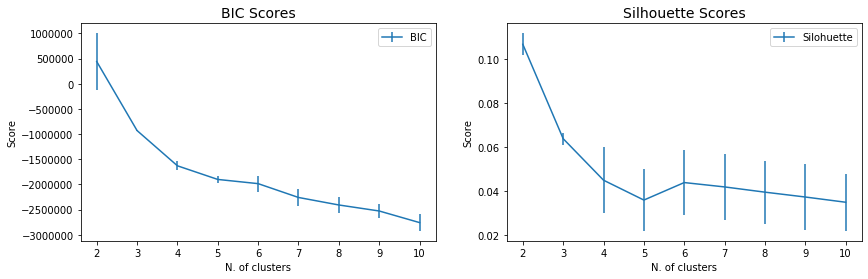
\includegraphics[scale=0.45]{graphs/output_39_0.png}
\end{center}
    
    
\paragraph{Silhouette score}
We can see the the bigger the number of clusters the higher standard
deviation. It turns out that we get the best score with 2 clusters. Also
3 clusters can be a candidate. if we consider the standard deviation
(the `error') of both configurations and the scores, 2 clusters is the
selected.

\paragraph{BIC score}
We can notice two things. The first is that the curve is fairly smooth
and monotone. The second is that the curve follows different slopes in
different part of it. Following this criterion, the bigger the number of
clusters, the better should be the model. Which means that the penalty
BIC gives to complex models, do not save us from over fit.

The slope in both scores at 2 and 3 clusters is most significant. The BIC score variance in 2 clusters is much more higher then 3. Hence 3 clusters is selected.

\section{Iterative GMM}
\subsection{Initialization}
\begin{verbatim}
GaussianMixture(covariance_type='full', init_params='kmeans', max_iter=100,
means_init=None, n_components=3, n_init=2, precisions_init=None,
random_state=42, reg_covar=1e-06, tol=0.001, verbose=0,
verbose_interval=10, warm_start=False, weights_init=None).fit(X)
\end{verbatim}

\begin{center}
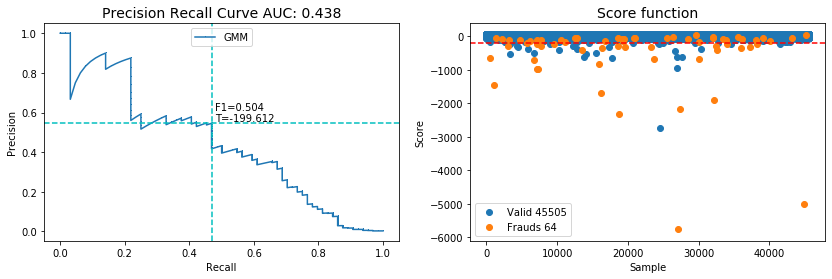
\includegraphics[scale=0.45]{graphs/output_48_0.png}
\end{center}
    
    It is very difficult to detect fraud transaction because in addition to
severe class imbalance there is also severe class overlap. Fraud
transactions are mixed with the valid ones in their log likelihood
score. It is important to tight our Gaussian model estimators to better
fit with the data. we will do it via our iterative approach(6) and
evaluate how better our Gaussian for detecting anomalies.\\
following results:

\subsection{Iterative}
\begin{center}
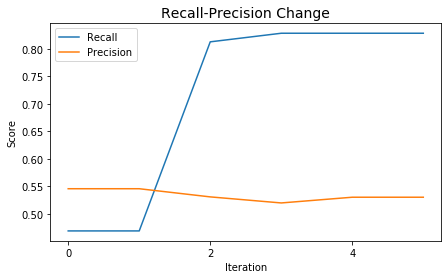
\includegraphics[scale=0.45]{graphs/output_52_0.png}
\end{center}
 We can observe that recall is increasing until converged to constant \textasciitilde{}0.8 while precision slightly switching between lower and upper bounds with a small slice until converged to constant \textasciitilde{}0.55. This is important because overall we do not harm model performance in each iteration. 
 
 Now we have the final model and we can select new threshold(5.2) $T$ with respect to precision-recall trade-off.

\subsubsection{Evaluate final model}

\begin{center}
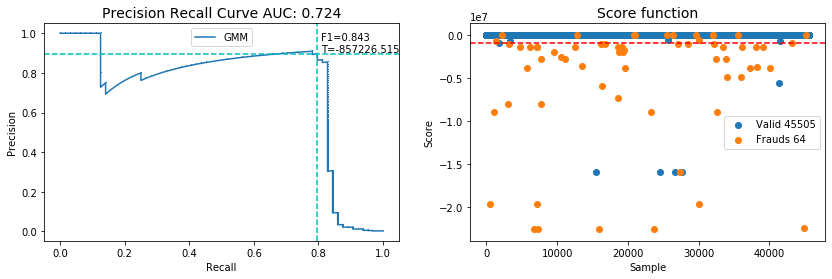
\includegraphics[scale=0.45]{graphs/output_55_0.png}
\end{center}
    
    Now it much more easy to detect frauds transactions based on log
likelihood function. Lower log likelihood function are indeed anomaly
transactions. We can conclude that our Gaussian estimators are more
fitted to valid transactions while we didn't fit the model only with
valid transactions!

\subsection{Evaluate test set}
    Testing model with test set achieved the following result:
                
    \begin{center}
        \begin{tabular}{ c c c c c}
          & precision & recall & f1-score &  support\\ 
         0 & 1.00 & 1.00 & 1.00 & 11374\\
         1 & 0.82 & 0.78 & 0.80 & 18\\
         \\
         accuracy & & & 1.00 & 11392\\
         macro avg & 0.91 & 0.89 & 0.90 & 11392\\
         weighted avg & 1.00 & 1.00 & 1.00 & 11392
        \end{tabular}
    \end{center}

\section{Iterative One Class SVM}
\subsection{Parameters}
\begin{enumerate}[label=\roman*)]
\item
  $\nu$: An upper bound on the fraction of training errors and a
  lower bound of the fraction of support vectors. Should be in the
  interval (0, 1). it is recommended to take $\nu$ near to the noise
  class, in our case frauds. we have imbalance data so we will set $\nu$ to
  0.01 which is 1\%.
\item
  $\gamma$: Kernel coefficient, gamma=`scale' is 1 / (n\_features * X.var())
\item
  $kernel$: RBF kernel functions selected they are should be good
  enough with our Gaussian distributed data.
\end{enumerate}

\subsection{Initialization}
\begin{verbatim}
OneClassSVM(cache_size=200, coef0=0.0, degree=3, gamma='scale', kernel='rbf',
max_iter=-1, nu=0.01, shrinking=True, tol=0.001, verbose=False).fit(X) 
\end{verbatim}
        
    \begin{center}
    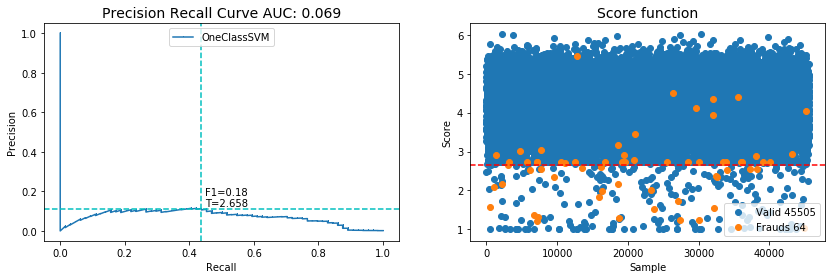
\includegraphics[scale=0.45]{graphs/output_65_0.png}
    \end{center}
    
    
    As we can see, OneClassSVM score function produced an area under the
threshold \(T\) that contain highly mixed area of valid and fraud
transaction. Here also it is very difficult to detect anomalies
transactions. We will try to better fit the support vectors estimators
with the iterative approach below.

\subsection{Iterative}
\begin{center}
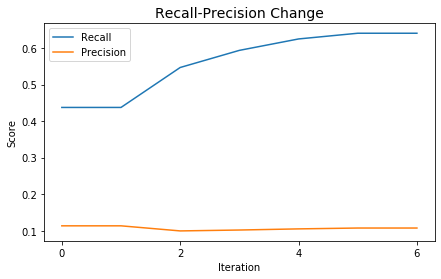
\includegraphics[scale=0.45]{graphs/output_69_0.png}
\end{center}

    Converged after the sixth iteration. We can observe that recall is increasing until converged to
constant \textasciitilde{}0.7 while precision stay constant with very
low percentage \textasciitilde{}0.1. Also here the iterative(6) approach do
not harm model performance in each iteration.

Now we have the final model and we can select new threshold(5.2) $T$ with
respect to precision-recall trade-off.

\subsubsection{Evaluate final model}

    \begin{center}
    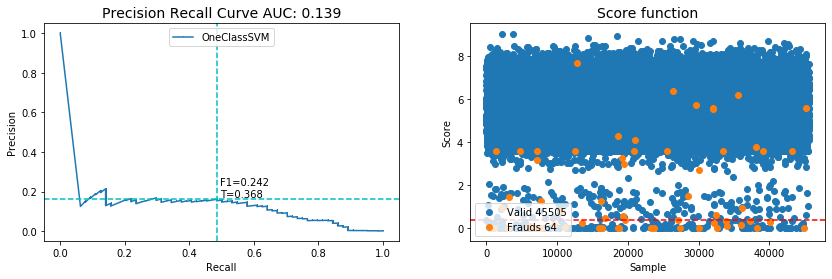
\includegraphics[scale=0.45]{graphs/output_72_0.png}
    \end{center}
    
    We got better result from initialization(9.2) in terms of valid-frauds spread
under the threshold \(T\), recall seems to be increasing to acceptable
value but precision keep low value.

\subsection{Evaluate test set}
Testing model with test set achieved the following results:
\begin{center}
    \begin{tabular}{ c c c c c}
          & precision & recall & f1-score &  support\\ 
         0 & 1.00 & 1.00 & 1.00 & 11374\\
         1 & 0.20 & 0.61 & 0.30 & 18\\
         \\
         accuracy & & & 1.00 & 11392\\
         macro avg & 0.60 & 0.80 & 0.65 & 11392\\
         weighted avg & 1.00 & 1.00 & 1.00 & 11392
    \end{tabular}
\end{center}

\section{Conclusion}
In this paper we propose a method that identifying frauds and pure valid transactions by assigning a score to each data point in highly imbalanced data set. The proposed method assumes no prior knowledge of either the frauds or valid transactions, don't do any features selection and fully unsupervised. We investigated the data, checked for data imbalance, visualized the features and understood the relationship and the dynamics between different features. The data was splitted into 2 parts, a train set and a test set. We trained Gaussian Mixture Model and OneClassSVM with real world credit card transactions data in an iterative method to achieve estimators fitted at possible to valid transactions. We showed that the models estimators getting better fitted in each iteration in terms of recall-precision. 

We can propose application such as to make recommendation for potential outliers for further investigation with high precision and recall and created training sets for novelty anomaly detection algorithms.


For summarize, Gaussian Mixture model obtained satisfying and acceptable results for the test set which can ensure to each part of the transaction processing chain a good protection from fraud and potentially chargebacks.
\end{document}
